% Income Shocks, Contraceptive Use, and Timing of Fertility
% incomeShocks-jde-r1.tex
% Begun.: 2017-07-13
% Edited: 2017-07-13

% Revisions based on Demography referee reports


\documentclass[letterpaper,12pt]{article}

\usepackage[title]{appendix}
\usepackage{amsmath}

\usepackage{fontspec}
\setromanfont[Ligatures=TeX]{TeX Gyre Pagella}
\usepackage{unicode-math}
\setmathfont{TeX Gyre Pagella Math}

\usepackage[margin=1.0in]{geometry}
\usepackage[figuresleft]{rotating}
\usepackage[longnamesfirst]{natbib}
\usepackage{dcolumn}
\usepackage{booktabs}
\usepackage{multirow}
\usepackage[flushleft]{threeparttable}
\usepackage{setspace}
\usepackage[justification=centering]{caption}
\usepackage[font=scriptsize]{subfig}
\usepackage[xetex,colorlinks=true,linkcolor=black,citecolor=black,urlcolor=black]{hyperref}
\usepackage{xfrac}

% Checking for unused references/labels - comment out before final run
% \usepackage{refcheck}

% \bibpunct{(}{)}{;}{a}{}{,}
\newcommand{\mco}[1]{\multicolumn{1}{c}{#1}}
\newcommand{\mct}[1]{\multicolumn{2}{c}{#1}}
\newcommand{\X}{$\times$ }
\newcommand{\hs}{\hspace{15pt}}

% Attempt to squeeze more floats in
\renewcommand\floatpagefraction{.9}
\renewcommand\topfraction{.9}
\renewcommand\bottomfraction{.9}
\renewcommand\textfraction{.1}
\setcounter{totalnumber}{50}
\setcounter{topnumber}{50}
\setcounter{bottomnumber}{50}


%------------------------------------------------------------------------


\title{Income Shocks, Contraceptive Use,\\ and Timing of Fertility\thanks{%
We would like to thank 
Alfredo Burlando,
Zo\"e McLaren, 
Erik Plug,
Lawrence Wu, 
two anonymous reviewers, 
and seminar participants at 
Agricultural Economics Society Annual Conference,
European Society for Population Economics Annual Conference,
IUSSP International Population Conference,
Montana State University, 
NEUDC 2015,
Norwegian School of Economics, 
Pacific Conference for Development Economics, 
the seventh annual PopPov Conference, 
Population Reference Bureau,
University of Oregon,
University of Washington,
and the 
Western Economic Association International Conference
for helpful comments and suggestions.
Partial support for this research came from a Eunice Kennedy Shriver National
Institute of Child Health and Human Development research infrastructure grant,
5R24HD042828, to the Center for Studies in Demography and Ecology at the
University of Washington.
}}

\author{Shamma Adeeb Alam\\
	Department of International Studies\\
	Dickinson College\\
	28 N College St\\
	Carlisle, PA 17013\\
	\href{mailto:alams@dickinson.edu}{\texttt{alams@dickinson.edu}}\\
\and
	Claus C P\"ortner\\
    Department of Economics\\
    Albers School of Business and Economics\\
    Seattle University, P.O. Box 222000\\
    Seattle, WA 98122\\
    \href{mailto:cportner@seattleu.edu}{\texttt{cportner@seattleu.edu}}\\
    \href{http://www.clausportner.com}{\texttt{www.clausportner.com}}\\
    \& \\
    Center for Studies in Demography and Ecology \\
    University of Washington\\ 
    }

\date{September 2017}

\begin{document}

% Need this for tables copied directly from estout
\def\sym#1{\ifmmode^{#1}\else\(^{#1}\)\fi}

\setcounter{page}{0}
\maketitle
\thispagestyle{empty}

\newpage
\setcounter{page}{0}
\thispagestyle{empty}

\doublespacing


\begin{abstract} 
% JDE abstract
\noindent This paper examines the relationship between income 
shocks and fertility decisions. 
Using panel data from Tanzania, we estimate the impact of agricultural shocks 
on 
pregnancies, 
births, 
and 
contraception use.
The likelihood of 
pregnancies and childbirth are significantly lower for households that experience
a crop shock.
Furthermore, women significantly increase their contraception use in response 
to crop losses. 
The increase in contraceptive use comes almost entirely from traditional 
contraceptive methods, such as abstinence and the rhythm method.
We argue that these changes in behavior are the result of deliberate decisions of
the households rather than the shocks' effects on other factors that influence
fertility, such as women's health status, the absence or migration of a spouse, 
the dissolution of partnerships, or the number of hours worked. 
We also show that, although traditional contraceptives have low overall
efficacy, households with a strong incentive to postpone fertility
are very effective at using them.

\noindent Keywords: Tanzania; family planning; shocks; timing of fertility

\noindent JEL codes: J1, 01, J2
\end{abstract}

\newpage


\section{Introduction}

How shocks affect fertility decisions in developing countries has 
received little attention in the literature.
A correlation between shocks and the timing of births is well-established, but it is 
unclear whether the cause is households' intentional planning or unintended consequences 
of the shocks \citep{pitt98b,lindstrom99,Evans2010,Portner2014}.%
\footnote{
There is a related literature on the effects of weather, especially temperature,
on timing of fertility \citep[see, for example,][]{Barreca2015}.
%  and TK Josh paper.
In a different vein, a monthlong blackout in Zanzibar increased 
births 8 to 10 months later \citep{Burlando2014}.
There is also a large literature examining how households in developing countries
cope with shocks in areas such as labor supply, crop choice, and education.
}
Furthermore, there is, in general, little evidence on what determines timing 
of fertility in developing countries, with most of the literature instead 
focusing on the number of children born \citep{Portner2018}.
% [Little evidence in general on timing of fertility in developing countries;
% most of the research has focused on completed fertility / children-ever-born] 
% Furthermore, standard models of fertility focus mainly on the effects of time
% invariant household and individual characteristics on fertility outcomes, and 
% tend to ignore the dynamic aspects of fertility decisions.%
% \footnote{
% For an early exception see \cite{Newman1984}.
% }

We seek to answer two key questions in this paper.
First, do income shocks, measured by accidental crop loss in Tanzania, affect the
timing of fertility?
Second, do changes in fertility timing, if any, arise from an intentional decision
to postpone fertility?

There are three reasons a household may want to delay fertility in the
event of a shock.
First, children are costly in the short run.
Having more children may eventually contribute to the household's production 
and help it overcome shocks, but the short-term impact on availability 
of resources is almost certainly negative \citep{Portner2014}.
Secondly, diverting time away from market work to child care will be even more 
costly if the household needs to respond to a shock by working more \citep{kochar99}.%
\footnote{
It is, however, also possible that a shock could temporarily lower women's 
cost of time, making it more attractive to have a birth now.
}
Finally, the household may realize that children born following a shock 
are more likely to be malnourished and have worse health outcomes, and therefore 
decide to postpone having the next child \citep{Portner2010}.

Observing a decline in pregnancies and birth rates following a shock is, however, 
not evidence of a conscious decision to change the timing of fertility.
A shock may, for example, lead one or more members of the household to 
migrate in search of better economic opportunities, and if either the husband 
or the wife are gone for extended periods, this will lower the probability of 
conception.
Furthermore, a shock may reduce intercourse frequency---either for
physiological or psychological reasons or from increased hours of work.
We would also observe a decline in births if people delay marriage or 
if there is an increase in the dissolution of marriage.
Finally, severe shocks can lead to starvation and health problems \citep{lindstrom99}.
Malnourished pregnant mothers are more likely to have stillbirths,
and non-pregnant women may see an increased incidence of secondary sterility
from a reduction in age of menopause or famine induced amenorrhea.%
\footnote{
See \cite{Hernandez-Julian2014} for a review of the literature and an 
analysis of the effect of famine on stillbirths.
}

Understanding the relation between shocks and fertility decisions is important for
three reasons.
First, as many households in developing countries experience a large number of shocks, 
it is important to understand the factors that help or hinder households' recovery 
after a shock.
Second, children born immediately after a shock fare worse than other children do.
In the short- and medium-term, they have worse health as measured by height-for-age 
Z-scores \citep{Portner2010}, and
long-term effects include worse self-reported health, lower schooling, and less
wealth \citep{Maccini2009}.
% This could be better explained
Finally, it helps us understand if, and how, households regulate their fertility.
% parents do not directly control fertility and its timing, but rather 
% control type and intensiveness of contraceptive use and the frequency and timing of 
% sexual activity.
This, in turn, can inform policies on availability and targeting
of family planning services.

Most of the prior literature on the impact of economic and other shocks on fertility 
has used historic data on what are now developed countries.
Data from Rouen, France, over the period 1681-1787, show that increases in the
price of wheat led to a dramatic fertility decline for the urban poor, 
whereas fertility of the urban wealthy was unaffected \citep{Galloway1987}.
Similarly, English data from 1542 to 1800 show that mortality shocks led to short-term
fertility declines, with the largest decline typically occurring  the year following 
the shock \citep{Bailey1998}.%
\footnote{
This data also indicated that an increase in real wage led to an increase in short-term 
fertility.
Increases in wage rate and declines in child mortality explain a significant part of the 
long-term fertility decline in Sweden during the period 1736 to 1946 \citep{Eckstein1999a}.
In another study on Sweden, increases in the value of women's time relative to men's 
time---arising from increases in the price of butter---led to a decline in fertility during 
the  1860-1910 period \citep{Schultz1985}. 
}
In pre-industrial Sweden, positive crop shock, positive weather shock, and 
positive wage shock all increased fertility for a five- to ten-year period following 
the shocks \citep{Eckstein1985}.
However, the increase in birth rate changed only the timing of births with no 
cumulative effect on the long-term fertility rate.
Similarly, the increasing price of rye in Southern Sweden led landless and 
semi-landless families to reduce their fertility, whereas landed farmers 
showed no change \citep{bengtsson06}.
Using present-day data, there is evidence that famine and domestic/regional 
military attacks in Ethiopia led to short-term decreases in the likelihood of 
conception \citep{lindstrom99}.
Closer to our paper, positive rainfall shocks in Senegal increased 
fertility \citep{pitt98b}.
None of these paper can, however, directly address whether the observed changes 
arise from deliberate control of fertility.

Many studies show how a variety of factors affect contraception use, such 
as, 
schooling, 
focused information campaigns, and
participation in savings or credit group 
\citep{Ainsworth1996,Feyisetan1996,Steele2001,Chen2003}.
To our knowledge, only one study attempts to show the effect of shocks on 
contraception use \citep{Hernandez-Correa2010}. 
Cross-sectional data from Madagascar show that households that experience adverse 
events are more likely to use contraception.\footnote{%
Adverse events include economic and environmental aspect, such as: rise in input 
cost, rise in cost of goods, difficulty finding buyers, difficulty finding inputs, 
floods, late rains, early rains, droughts, pest problems, etc. 
} 
However, 
% households may be able to anticipate many of these events before 
% they occur and adjust their behavior accordingly.
% Furthermore, 
the possible correlation between the probability of experiencing 
an adverse event and unobserved individual and household characteristics may 
bias the estimates, and the cross-sectional data allows for neither household 
nor individual level fixed effects estimates.

We use longitudinal data from the Kagera region in Tanzania with information on 
accidental crop loss, fertility, and contraceptive use to estimate individual 
level fixed effects models of the effects of income shocks on both timing of 
fertility and contraceptive use.
We show that income shocks decrease the likelihood of pregnancies and births.
At the same time, shocks significantly increase use of contraceptives.
This increase mainly occurs through the use of traditional contraceptives, 
which are the dominant form of contraception in the area.
We argue that the postponement of fertility in households experiencing income 
shocks is the result of the increased contraception use rather than a biological 
response or separation of spouses.

The paper makes three main contributions to the literature. 
First, this is the first paper to show that households respond to income shocks 
through contraceptive use, which, in turn, affects the timing of child bearing. 
% Our study provides evidence that the postponement of fertility occurs through a 
% planned decision process rather than as an unplanned consequence.
Second, with low rates of modern contraceptive use in the area, the paper contributes 
to the literature on how populations control fertility before widespread adoption of
modern contraception.%
\footnote{
There has long been a discussion of when and how families 
undertook fertility control before the emergence of modern 
contraceptives \citep{Guinnane2011,Cinnirella2017}.
Simulations show that it clearly is possible to substantially limit fertility
even with only access to traditional contraceptives, but there is only 
limited evidence available on exactly which methods were actually used 
\citep{Michael1976,David1986,Santow1995}.
}
Finally, the paper contributes to the consumption smoothing literature, as households 
affected by income shock use family planning as a mechanism to smooth their consumption. 
In the short run, bearing a child means diverting scarce resources away from other
useful purposes to the birth and maintenance of the child. 
Farmers can, therefore, partly smooth their consumption by delaying births during 
times of income shock.



\section{Data and Estimation Strategy}

We use the Kagera Health and Development Survey (KHDS) conducted by the World Bank 
and the University of Dar es Salaam in the Kagera region in Tanzania. 
The survey covers four rounds from 1991 through 1994 and over 800 households, 
drawn from 51 communities (49 villages) in the six districts of Kagera.%
\footnote{
The sample selection was based on a variable probability sampling procedure 
(a two-stage, randomized stratified procedure) based on expected mortality.
In the first stage, based on the 1988 Tanzanian census, the census clusters were randomly 
selected after stratifying them according to mortality rates and agro-climatic zones. 
Households were then divided into ``high-risk'' and ``low-risk'' groups in the 
second stage, based on illness and death of households in the 12 months 
before the enumeration process.
Finally, households were randomly sampled from the groups.
For further details on the sample selection, see World Bank (2004).
}
The average interval between each of the survey round was between six and seven months, 
and interviews of households took place on a rolling basis throughout the year. 
The Kagera region is in the northwestern corner of Tanzania, west of Lake Victoria, and 
borders Uganda, Rwanda, and Burundi. 
The population of the area---1.3 million in 1988---is 
overwhelmingly rural and primarily engaged in agriculture. 


% \begin{figure}[ht] 
%  \centering
%  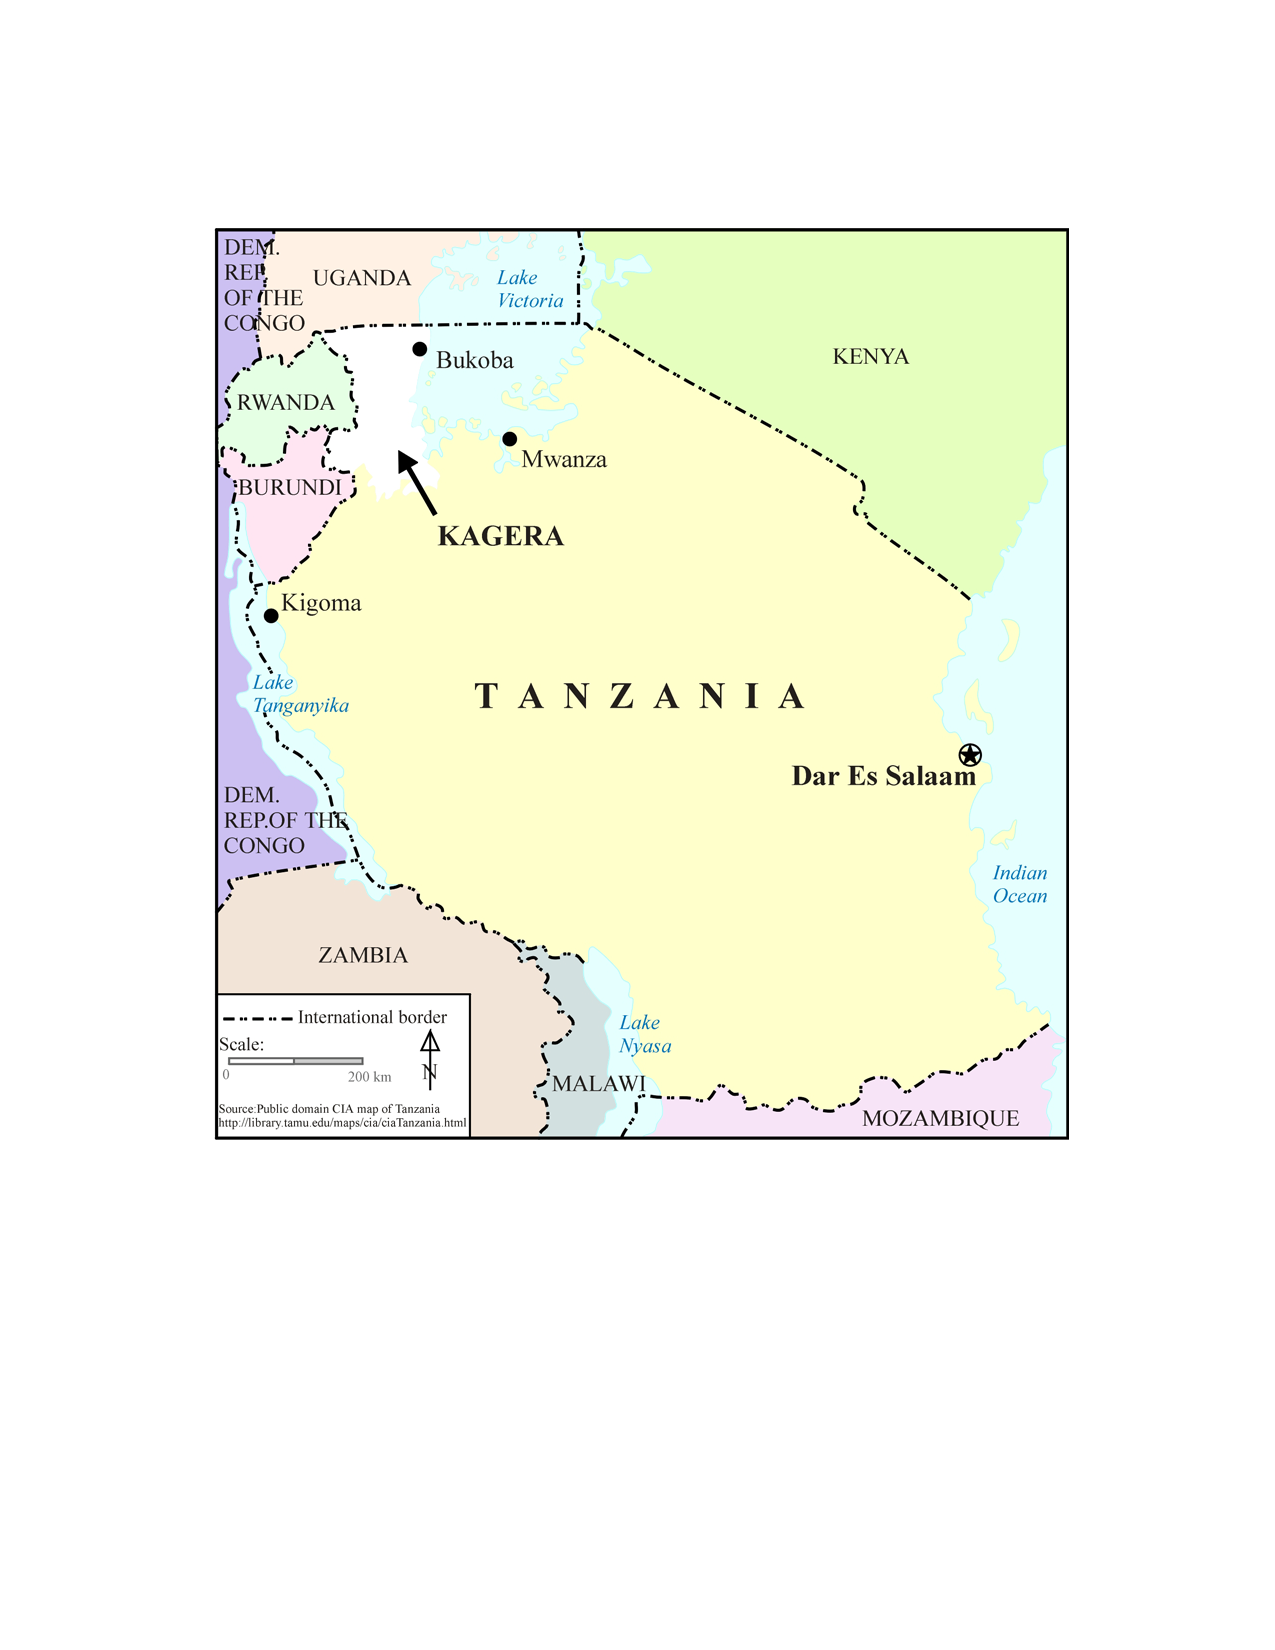
\includegraphics[width=0.6\textwidth]{../staticPDF/kagera.pdf}
%  \caption{Map of Kagera region}
%   \label{fig:kagera_map}
% \end{figure}


The data contain information on individual and household level demographic 
and socio-economic characteristics. 
In addition, questions about fertility and birth control were asked of all 
married women, regardless of age, and unmarried women 14 years and older. 
We restrict our sample to married or partnered women 17-45 years of age who we 
observe in all 4 rounds of the survey.
This ensures that we capture women who are at risk of conception and for whom 
the available observations cover sufficient time for shocks to have an effect
on pregnancies and births.
The downside is that the sample size is reduced.
We discuss possible non-random attrition below.

% Descriptive statistics by wave
\input{../tables/desstat2.tex}



Table \ref{tab:desc_stat_croploss} shows the main explanatory variable of interest 
and the 5 outcomes that we examine.
The main explanatory variable is a dummy for whether the household experienced 
an accidental loss of crops, which covers any crop lost due to insects, 
rodents, fire, rotting, or other calamities, greater than TZS 200 since the 
prior survey round (or prior 1 year for the first round).
There is substantial variation in the number of households that experience a 
crop loss between the 4 survey rounds.
In the 12 months prior to the first survey just below 70\% of households 
lost crops, whereas 25\% lost crops between the 1st and 2nd surveys.
That falls even further for the 3rd and 4th rounds, with less than 3\% 
reporting crop loss of more than TZS 200 for both.
The TZS 200 cut-off is equivalent to approximately 5th 
percentile of all household savings.
Our results are robust to alternative definitions of crop loss as we
discuss in Section \ref{sec:robustness}.


On average across the four surveys, 17\% of women report being pregnant 
at the time of the interviews and 16\% of women report giving birth since the 
prior survey round.
In total, just below 70\% of women in the sample report giving birth in
the covered period (approximately 3\sfrac{1}{2} years).
Similarly, 70\% report a pregnancy at one point during the 4 rounds.


We capture contraceptive use at the time of the survey, and further divide
contraceptives into traditional and modern types. 
Traditional contraceptives include abstinence, rhythm, and withdrawal, 
and modern contraceptives include condom, diaphragm, pill, IUD, injection,
and female and male sterilization.%
\footnote{
The relevant question is "Some couples use contraception methods to avoid
pregnancy or to space births. Are you currently using a method of contraception?"
If the woman answers yes, she is then asked "What contraceptive method are you
and your partner using at present?"
}
A small subset of women report using both modern and traditional contraceptives;
these women are included in both categories.
If a woman is currently pregnant, we code her as not using contraceptives.
We remove sterilized women from the sample, as sterilization is typically a 
permanent procedure.

Contraceptive prevalence is low; at the time of the first survey round, 14\% 
of women report using any type of contraceptive---split between 11 percent that use 
traditional contraceptives and 4\% that use modern contraceptives.
In subsequent survey rounds, the contraceptive use rate is just below 10\%, 
with 4 to 6\% using traditional contraceptives and 2 to 5\% 
using modern contraceptives.


% [Descriptive statistics and discussion here]
\input{../tables/desstat1.tex}


Table \ref{tab:desc_stat_women} shows descriptive statistics for basic
demographic and household characteristics at wave 1.
As the time span of the surveys is too short to confidently identify age effects,
we use women's age at the time of the first survey round.
There is substantial measurement error in age and heaping of reported ages 
around numbers ending in 0 and 5.%
\footnote{
Some women report the same age in all survey rounds despite that there are
21 months between the first and last survey round, whereas other women's reported 
age goes up by 1 year between each survey round despite that the surveys are only 
6 to 7 months apart.
}
We use respondent's median reported age, rounded down, and 5-year age groups 
centered around ages ending in 0 and 5 to take account of heaping.
Only married/partnered women are in the sample, which explains the 
equal age distribution despite population growth in the area.

A notable characteristic is the high level of reported education for a poor 
rural area, although there also appears to be errors in 
reported education levels.%
\footnote{
For many women, the reported education level decreases in certain survey 
rounds, or increases by 2 years or more in consecutive survey rounds, which 
conflicts with the 6 to 7 months survey intervals. 
Additionally, individuals are supposed to complete primary school by the age of 15,
so changes in primary schooling levels in our sample is likely from reporting 
errors. 
For women who report different primary school education levels, we 
assign the modal education level if possible, or, if there is no modal 
observation, the median years of education.
We use the same approach for household heads' education
when we use household heads' education as a proxy for wealth.
}
We divide education levels into three groups: no education, 
some primary (1-6 years of education), and primary school 
or above (7 or more years of education).
Only 29\% of the women received no education, 27\% received some 
primary education, and 44\% completed at least primary education.
The high reported education level is most likely the result of the 1974 
Universal Primary Education Movement,
which increased accessibility of primary education and enrollment rates, 
even though there are reports that the quality of education was very low.%
% In addition, the crisis Tanzania experienced in the 1980s further lowered the 
% quality and enrollments declined significantly.%
\footnote{
See \cite{Galabawa2001} and \cite{Wedgwood2005} for detailed discussions 
of the development of education in Tanzania.
}
Hence, it is unclear to what extent reported education levels reflect 
women's actual human capital.

Finally, to capture wealth status of the household, we use total reported assets of the 
household.
These include self-reported values of land, livestock, business assets, durable
goods, and savings.
The average level of assets in wave 1 was TZS 70,000.%
\footnote{
In 1991 the official exchange rate was TZS 200 to the dollar, while it
was TZS 440 to the dollar in the parallel market.
}
There was, however, wide dispersion in asset levels, with the minimum reported 
wave 1 asset level around TZS 500 and the maximum almost TZS 1,100,000.
The 25-percentile asset level is below TZS 19,000, median is approximately 
TZS 34,000, and the 75-percentile asset level is only slightly higher than the 
mean at TZS 71,500.
In other words, the asset levels for the majority of households is 
very low, with a few relatively wealthy households.

A potential issue is that some women may be left out of our sample because of
non-random attrition.
In Appendix Tables \ref{tab:attrition_desc_stat_croploss} and 
\ref{tab:attrition_desc_stat_women}
we show descriptive statistics for women who fulfilled the requirements for being in the 
sample in wave 1, but were not included in the main sample.
A total of 164 women were dropped because they were not observed in all four waves 
and/or failed the criteria in at least a one of the later waves, for example 
because they divorced or became widows.%
\footnote{
Divorce, separation, and widowhood accounted for 22 women, whereas not observed in all
4 waves for accounted for 147 women. 
The two numbers do not add to 169 because some women experienced both a change
in marital status and were not observed in all 4 waves.
}
In each period, women who were dropped from the sample were less likely to have 
been affected by a shock.
Furthermore, they were slightly less likely to be pregnant and to have given 
birth, and, correspondingly, a larger percentage use contraceptives.
Compared to our main sample the women dropped were more likely to be young,
with 10 percentage points more in the very youngest age group and 3 
percentage points at the second youngest age group.
They were also more educated and had a slightly higher level of asset per capita.
Hence, it appears that we are not dropping women who were more likely to 
experience shocks and less likely to cope with them.
However, to further investigate possible non-random attrition, we 
estimate the association between shocks and partner migration and between
shocks and dissolution of marriage below.



\subsection{Estimation Strategy}

An important concern when estimating
the effects of shocks on fertility and contraception decisions 
is that there may be unobserved factors that affect both likelihood of 
shocks and outcomes.
A household with lower (unobserved) ability may, for example, simultaneously be more 
likely to experience a shock and less likely to afford or have knowledge about 
contraceptives.
This would bias OLS estimates of shocks' effects towards zero.
To address the problem of unobserved heterogeneity and endogeneity, our
preferred model is an individual level fixed effect model. 
This approach allows us to control for all time-invariant mother characteristics when 
estimating the impact of crop loss on contraceptive use and fertility outcomes.
The main downside is that fixed effects tend to exacerbate measurement errors.

We estimate OLS and community and individual level fixed effects 
versions of equation (\ref{eq:fixed_effects1}),
\begin{align}
Y_{i,t} &=  \beta_1 S_{i,t}  + \alpha_{t} 
+ \mu_i + \varepsilon_{i,t},   \label{eq:fixed_effects1} 
\end{align}
where $Y_{i,t}$ is the outcome of interest,  
$S_{i,t}$ is whether the household experienced a shock in the relevant period,
$\alpha_{t}$ is a vector of survey wave dummies, 
and $\mu_i$ is time-invariant individual specific characteristics.
With the outcomes of interest all dichotomous, the estimated equations 
are linear probability models.
 
For the outcome variables, currently pregnant and contraceptive use, we use 
a dummy variable for crop loss that occurred in the period immediately 
prior to the interview, which is 6 to 7 months long, as our main explanatory 
variable of interest. 
When birth is the outcome variable, 
we use a dummy variable for crop loss that occurred in the period between 
the prior two survey rounds.%
\footnote{
In the tables we indicate this difference by referring to the period 
immediately before the survey as 1-7 months and the period between the
prior survey and the survey before that as 7-14 months.
}
The reason for the longer lag is that with an average gestation period
of 9 months only crop losses that occurred longer ago are relevant.%
\footnote{
It is possible that the most recent crop loss could impact the likelihood
of carrying a pregnancy to term, although this would require severe
food deprivation \citep{Hernandez-Julian2014}.
We investigate this possibility indirectly when examining the effects
of crop loss on health.
}


\section{Results}

% [BASELINE estimations]

First, we address whether agricultural shocks affect timing of fertility at all.
Table \ref{tab:birth} shows OLS, community fixed effects, and woman level individual 
fixed effects estimates of the effect of crop loss on the likelihood of pregnancy 
and childbirth.
The three left columns show the effects of crop loss in the 7 months prior to the
survey on a woman's likelihood of being pregnant at the time of the interview.
The three right columns show the effects of crop loss on the likelihood of having given 
birth since the last survey round. 
For a birth to have occurred in the 7 months prior to the interview, a woman would have
had to conceive in the period before the prior survey round, and we therefore use shocks
that occurred 7 to 14 months prior to current round.


% health effect explain the difference between births and pregnancy.
% We would also expect pregnancy to be a little lower because some women may not
% realize that they are pregnant. 
% 95\% pregnancy: -.1774091   -.0084771
% 95\% birth: -.2570566   -.0607087

% Table with pregnancy and birth results
\input{../tables/main_pregnant_birth.tex}

Two main results stand out.
First, there are statistically significant and negative effects of crop loss on the
likelihood of both pregnancies and births.
Our preferred estimates---woman level fixed effects---show that experiencing 
crop loss decreases the likelihood of being pregnant by 10 percentage points 
and the likelihood of a birth by 17 percentage points.
These effects are substantial; on average across the four survey rounds, approximately 
17\% of women were pregnant and 17\% had given birth in the preceding period. 
Second, the absolute values of the community fixed effects point estimates are 
larger than the OLS estimates for both outcomes and the individual level
fixed effects estimates are larger than the community fixed effects estimates.%
\footnote{
Full results for the OLS and community fixed effects models are in shown in 
Table \ref{tab:ols_fertility}.
Table \ref{tab:com_cluster_birth} shows the results with clustering at community level
to account for potential spacial correlation in shocks.
Clustering at community level leads to slightly lower statistically significance 
for pregnancies and slightly higher statistically significance for births.
}
This suggests that unobservable characteristics, at both community
and individual level, correlate with a higher likelihood of experiencing 
a shock and lower likelihood of using contraceptives.


% Table with contraceptive use results
\input{../tables/main_contraceptives.tex}


Our results in Table \ref{tab:birth} are consistent with the prior literature,
with shocks associated with statistically significant declines in pregnancies 
and births.
But, households do not control these two outcomes directly.
Instead, they have control over some of the proximate determinants of fertility, 
such as use of contraceptives and coital frequency.
Our second question is to what extent households are intentionally delaying 
the conception and birth of their next child. 
To answer this question, we examine the effects of crop loss in the 7 months
prior to the survey on contraceptive use at the time of the interview. 
Table \ref{tab:contraceptive} presents OLS, community fixed effects, and woman 
level individual fixed effects estimates of  effect of crop loss on overall 
contraceptive use and use by type.%
\footnote{
Full results for the OLS and community fixed effects models are in shown in 
Table \ref{tab:ols_contraceptive}.
Table \ref{tab:com_cluster_contraceptive} show results with clustering at
community level, which leads to little change in the level of
statistically significance.
}

The main result is that crop loss leads to a statistically significant 
increase in the overall contraceptive use.
Our preferred model shows that crop loss is associated with
an almost 8 percentage points increase in contraceptive use.%
\footnote{
The difference between the OLS, community, and individual level fixed effects
estimates are consistent, but less clear-cut, with what we found for pregnancies 
and births.
The woman fixed effects estimate is again the largest.
}
The effect on overall contraceptive use is substantial considering that the 
average use rates across the four rounds vary between 8 and 14\%.
The statistically significant increase in contraceptive use following
a crop loss indicates that households are reacting to crop 
losses by increasing contraceptive use.

Splitting contraceptive use into traditional and modern shows that almost
all of the increase in contraceptive use comes from traditional contraceptives.
The individual fixed effects specification shows that a
crop loss leads to a statistically significant increase in
traditional contraceptive use by 6.2 percentage points, whereas
the effect on use of modern contraception is 2 percentage points
and not statistically significant. 
Given the low levels of use for modern contraceptives in the area
this result is not surprising.

In sum, crop loss is strongly associated with a decline in
both the likelihood of being currently pregnant and the likelihood
of having given birth in the period before the survey round.
Furthermore, women who experienced a crop loss are substantially
more likely to use contraceptives, especially traditional methods.
These results are consistent with the idea that households 
deliberately postpone births in response to adverse shocks.

\subsection{Conscious Decision or Unintended Consequence?}

Our main results point to households making a conscious decision
to postpone fertility in the face of a shock.
Three questions arise from our results.
First, 
why are there differences in the point estimates for
the effects of crop across the three main outcomes: 
births, pregnancy, and contraceptive use?
Second, 
are we picking up behavior changes brought on by
crop loss---such as decrease in coital frequency from poor
health or a substantial increase in hours worked---that is later 
rationalized or reported as increased use of traditional 
contraception methods such as abstinence?
Third, 
how can the effect on postponement of fertility be so
strong if traditional contraceptives have low efficacy?
We attempt to answer these questions in this section.

The first question is why the point estimates for the three main 
outcomes differ.
If deliberate timing of fertility was the only explanation, 
we should observe similar absolute effects of crop loss across all three outcomes.
But, the point estimate is largest for births, second largest for pregnancy, 
and smallest for contraceptive use.
Part of the explanation for this could be simple random variation.
Indeed, we cannot reject that the absolute values of the point 
estimates for pregnancy and contraceptive use are the same, 
although we can reject that the point estimates are the same
at the 5\% significance level for births and pregnancy and at
the 10\% level for births and contraceptive use.%
\footnote{
The tests were done using Stata's ``suest'' command, which allows for correlation 
of errors across the three main fixed effects models,  with clustering at
household level. 
}

The pattern of largest point estimate for births, followed by
pregnancy and contraceptive use also matches what we would 
expect to arise from measurement error.
As mentioned above, fixed effect models exacerbate measurement error, 
which bias the estimated coefficients toward zero.
Of the three outcomes, births should have the least amount of 
measurement errors.
Women know whether they have given birth, 
although it is possible that some women report a birth that occurred 
before the prior survey and others fail to report births that 
occurred between the prior survey and the current one.
Pregnancy is associated with more measurement error;
some women may believe themselves to be pregnant when they are
not and some women may not realize that they are pregnant.
Contraceptive use likely has the most measurement 
error---especially in relation to how we measure births and pregnancies.
The surveys asked only about current use, so some women may
have used contraceptives intensively since last survey and 
just recently stopped, or only recently begun.
Obviously, we cannot verify that measurement error is the explanation.
It is, however, consistent with crop loss having the same underlying impact on 
all outcomes, with measurement error biasing the estimated effects most 
for contraceptives and least for births.
What also points in this direction is that the OLS point estimates 
are even less statistically significantly different from each other
than the fixed effects point estimates.%
\footnote{
Of course, the problem with the OLS estimates is that they
do not adequately control for endogeneity, although we see
no strong reason why this should be related to differences
in the degree of measurement error across the three outcomes.
}

Finally, it is possible that the differences in point estimates 
could reflect effects of crop loss other than conscious 
delay of fertility.
There are two main possible culprits: a decline in health
or the absence of the husband or the wife.
Worsening health has three effects.
First, more women will be unable to conceive, which would make
the effect of crop loss on pregnancy larger than the effect
on contraceptive use.
Second, those women who do conceive will be less likely to carry their 
pregnancy to term, which would make the effect on births 
larger than the effect on pregnancy.
Third, worse health could lead to lower coital frequency,
which is also consistent with larger effects on births and
pregnancy than on contraceptive use.
Similarly, the absence of a partner will lower the risk of
pregnancy and birth for a given level of contraceptive use.



% Table with pregnancy and birth results
\input{../tables/main_health_marriage.tex}



Table \ref{tab:health} shows the impacts of crop loss on body mass index 
(BMI) and self-reported illness in the last 4 weeks for the women, 
outmigration of partner, and risk of marriage dissolution. 
Both health outcomes have the expected signs, but the effects are small
and not statistically significant, making it unlikely that it 
would be associated even with a sufficient reduction in 
coital frequency to explain the results.
Similarly, Table \ref{tab:health} shows that shocks do not lead to a
significant increase in migration or a significant increase in dissolution of
marriages.
The coefficient for migration has the expected positive sign, but the
effect is too small to explain the reduction in pregnancies and births. 
In contrast, the coefficient for dissolution of marriage has the
opposite sign, and the magnitude is near zero. 
Hence, neither health nor the absence of a partner seem to drive the
postponement of fertility, suggesting that the effect of crop loss 
works predominately through the increased use of contraceptives.


% - hours worked and abstinence  / also shows that the shocks are "real"
In addition to health related reductions in coital frequency, 
it also possible that the amount worked increases so substantially 
that coital frequency declines and the respondent reports this as abstinence.%
\footnote{
We are grateful to Lawrence Wu for suggesting this mechanism.
}
% We examine this possibility in two ways.
% First, 
For this explanation to hold the amount worked must increase 
dramatically.%
\footnote{
As we mentioned in the introduction it is possible that crop loss could
decrease labor supply, especially if households mainly provide labor
to their own land and there are imperfect labor markets.
A decrease in labor supply is, however, likely associated with an
increase in fertility.
}
We estimated the effect of both the dummy for crop loss and the log
of crop lost on hours worked per week for women in our sample.%
\footnote{
Appendix Table \ref{tab:hours} shows the results.
}
A shock does, indeed, increase the hours worked per week, but the 
effect is only slightly above 1 hour for the dummy measure of crop loss, 
and that effect is not statistically significant.
Using log of crop loss, the effect is statistically insignificant
and the effect is still relatively small; 
a 1\% increase in the size of a crop loss leads to a 0.05 hours
increase in amount worked per week.
In sum, combined with an average work week of just below 44 hours a week,
it is unlikely that a substantial amount of the reduction in 
fertility is explained by lower coital frequency brought on by
high work load.

% Second, we can disentangle the different types of contraceptives.
% Given the small sample size this is, however, at best suggestive.
% Excluding abstinence, the effects of crop loss on contraceptive use
% are smaller and just above the 10\% significance level.
% The effect on abstinence only is almost the same size, but that
% effect is statistically significant at the 5\% level.%
% \footnote{
% Appendix Table \ref{tab:excludeAbs} shows the results.
% }
% With the relatively low use rates of modern contraceptives, this
% is not surprising given that abstinence is clearly the only 100\%
% effective traditional contraceptive.

% Third, 
% how can the effect on postponement of fertility be so
% strong if traditional contraceptives are generally considered 
% to be of low efficacy?

The final question is how the effect on postponement of fertility 
is so strong when there is little use of modern contraceptives.
In Table \ref{tab:effectiveness}, we examine to what extent shocks cause
a delay in pregnancy through the increased use of contraceptives by
estimating the following: 
the effects of crop loss between the prior survey and the
survey before that, contraceptive use at the prior survey round, and their
interaction on whether the respondent is currently pregnant.
Contraceptive use is clearly endogenous, but this can provide 
suggestive evidence on whether shocks do delay
pregnancy through increased use of contraceptives. 

% Table with contraceptive use effect on pregnancy
\input{../tables/main_effectiveness.tex}


Crop loss, by itself, has a small, not statistically significant,
and positive association with pregnancy.
Using contraceptives is associated with large and statistically 
significant, but \emph{higher} likelihood of pregnancy.
The interaction term of crop loss and contraceptive use is,
however, negative, large, and statistically significant. 
With the caveat that contraceptive use is endogenous, this suggests
that women using contraceptives following a crop loss are significantly 
less likely to be pregnant. 
In order words, once there is a strong enough incentive to avoid
becoming pregnant, traditional contraceptives have a surprisingly high
effectiveness rate.%
\footnote{
The statistically significant and large positive effect of 
contraceptive use by itself it likely the result of capturing
that these women are also the most likely to be sexually active.
Appendix Table \ref{tab:abstinence} shows the association 
between crop loss, contraceptive use, and current pregnancy with 
contraceptive use split by abstinence only, other traditional
contraceptive use, and modern contraceptives.
With the caveat that the low number of observations for each use 
makes it difficult to draw strong conclusions, it appear that
abstinence is the most ``effective'', followed by modern
contraceptives, whereas other traditional contraceptive interacted
with crop loss do not have a statistically significant association.
}
This also suggests that the crop loss is affecting conceptions primarily 
through contraceptive use, and not through some other channel.



\subsection{Robustness of Results\label{sec:robustness}}

Finally, we discuss a number of robustness checks for our results.
The most important concern is our definition of crop loss.
Above we define crop loss as a loss of more than 200 TZS.
To check how sensitive our results are to this cut-off,
we re-ran the regressions with varying cut-offs from 
0 to 5,000 TZS.%
\footnote{
The results are shown in Appendix Table \ref{tab:cut_offs}.
}
The signs of the coefficients are the same across all cut-offs.
Between 100 and 1,000 TZS, crop loss has a statistically significant
effect on same outcome as above.
Above 1,000 TZS the effects on pregnancy and birth become smaller and 
eventually statistically significant insignificant.
This is not surprising.
With a higher cut-off, more and more households will have experienced 
a crop loss but are not counted as having one, which will tend to 
bias results towards zero if crop loss have an effect at levels 
lower than the cut-off.%
\footnote{
This is supported by regressions---not shown---where we drop all observations 
with crop loss larger than zero but smaller or equal to the cut-off and find 
substantially larger coefficients.
} 
Using the log of crop loss instead of a cut-off does
not change our conclusion that crop loss significantly reduces
the likelihood of a pregnancy and birth and significantly
increases the use of contraception.%
\footnote{
See Appendix Table \ref{tab:ln_croploss}.
Using continuous crop loss leads to similar signed coefficients,
although neither pregnancy or birth are statistically significant
as shown in Appendix Table \ref{tab:continuous}.
Given the unattractive assumption that the effect of an unit
increase in crop loss is the same at all levels inherent in
this specification, the lack of statistically significance is
not surprising. 
}
The same is the case if we use a Logit model instead of the
linear probability model.%
\footnote{
See Appendix Table \ref{tab:logit}.
}

% Trend (based on R2 question)
A potential concern with the data is the large differences in
the number of households that experience a crop loss across
the waves.
One possibility is that our results are driven by a time
trend that affect households that are more likely to
experience crop losses.
We use two models to investigate this possibility.
First, we interact a linear time trend with wave 1 characteristics 
(assets per capita, age group dummies, and education group dummies).
Second, we interact wave dummies with the same set of wave 1 
characteristics.%
\footnote{
The results are shown in Appendix Table \ref{tab:timetrend_birth}.
}
The differences from the original results in point estimates 
and levels of significance are minimal, indicating that 
our results are not driven by differential trends in which 
types of households that experience crop loss.

% combine these two questions
% Omitted variables (based on R2 question)
% Time varying results (based on R1 question)
Furthermore, our definition of crop loss is based on the 
household's assessment and cannot be directly verified.
It is therefore possible that omitted, time-varying 
factors are responsible for the results. 
We approach this issue in two ways.
First, we included two other time-varying factors that
may affect fertility, loss of livestock and a price
index, in the main regressions.%
\footnote{
See results in Appendix Table \ref{tab:timevarying}.
Note, that the loss of livestock unfortunately also
includes livestock given away by the household.
}
Neither of these variables are statistically significant
and the coefficient on crop loss does not change.
[TK bla, bla - next sentences need a rewrite]
Although this does not completely rule out the possibility
that other time-varying factors, such as an epidemic or
local conflict, could affect fertility decisions, it does
imply that unobserved time-varying factors were not a 
major influence.
Conflict and epidemics would most likely have had 
substantial effects on either or both of the new
time-varying variables included.

Second, we examined if rainfall predicts crop loss.%
\footnote{
See Appendix Table \ref{tab:rainfall}.
}
Higher rainfall is significantly associated with a 
lower risk of crop loss,
% , a dummy for missing
% information on rainfall is also substantially 
% associated with crop loss.
% Furthermore, 
although including rainfall as an additional
variable in the main regressions did little to
change the estimated effects.


% - Something else changes in the village
It is also possible that crop loss results in spill-overs to other
households.
We therefore added the fraction of households that experienced a crop
loss in the community---over both the last 7 months and the period 
between the two prior surveys---to the specifications.%
\footnote{
This fraction is calculated on the complete sample of households
rather than the sample of women used here.
Results are shown in Appendix Table \ref{tab:vill_croploss}.
}
The effects of crop loss on pregnancy and birth are slightly smaller,
although the levels of statistical significance remain the same.
The effects of any contraception use and use of traditional
contraception are both lower, with the effect on traditional
contraception no longer statistically significant.
Only for traditional contraception use is the village level 
coefficient statistically significant.
Another way to look at this is that the spillovers from other
households' exposure to shocks are generally not large enough to 
force not exposed households to change their fertility and 
contraceptive behavior.

% - preemptive behavior (pregnant / contraceptive use predict shocks) 

Households may also anticipate shocks and
change their behavior in response to the expected shocks.
One way to examine this is to reverse the estimations.
We therefore estimate whether contraceptive use at the time of the last 
survey was associated with observing a crop loss between the last survey
and the current one and similarly for pregnancy at prior survey and 
birth in the period before the prior survey.%
\footnote{
Appendix Table \ref{tab:reverse} shows the results.
We examine both the dummy for crop loss and the log of crop loss.
}
There are no statistically significant direct effects of 
prior behavior on current crop loss, measured as either a
dummy or log of amount of crop loss.
The small effects and lack of statistical significance 
indicate that crop losses are, indeed, unanticipated 
shocks.

% Other results

[TK This last part is crap!]

Finally, the Appendix discuss in detail whether the results 
vary by age group, wealth, and education levels.
None of these lead to strong conclusions on how crop loss 
affect fertility decision by household and individual
characteristics.
The Appendix also discuss how including additional lags
of crop loss affects the results.
In principle, if shocks lead to a postponement of fertility we 
should see longer lags be associated with higher fertility, 
whereas if shocks lead to a permanent reduction in fertility we
should not see any compensatory effect.
There are, however, a number of issues with this approach.
First, it is possible that the effect of a crop loss is felt
in subsequent period and not only in the period in which it
was observed.
Second, longer spacing between births can be costly because economies
of scale are harder to realize and because the mother may have to 
be out of the labor force for longer if she already have young
children to care for.
This implies that a household that are hit twice in a row by
a crop loss is likely to behave differently from a household that
is hit once.
Both of these factors make it difficult to draw strong 
predictions on what the effects should be (except that the
initial impact should lead to postponement of fertility).





\section{Conclusion}

We estimate the relationship between household income shocks and decisions
on timing of fertility. 
To account for potential correlation between unobservable household
characteristics and both shocks and fertility decisions, we employ a fixed effect model.
Our estimates show that both the likelihood of pregnancy and birth decrease in
response to a crop loss and that contraceptive use, especially use of traditional 
methods, such as abstinence and rhythm, significantly increases. 

We examine a number of causes that may explain the reduction 
in fertility following a crop loss.
Crop loss shocks do not worsen women's health enough to 
reduce pregnancies and childbirths to the extent that we find.
Furthermore, with no significant change in the likelihood of migration or 
dissolution of partnership in response to crop loss, there is no evidence 
that the reduction is due to physical separation of spouses or partner.
As expected, the number of hours worked increases for women after a shock, 
but the effect is unlikely to be large enough to affect fertility 
through a change in coital frequency.

Our main conclusion is that households consciously delay 
fertility through contraceptive use to cope with income shocks. 
This is especially of interest since this is accomplished 
predominately through the use of traditional contraceptives.
If traditional contraceptives have low efficacy, a natural question is 
how the substantial reductions in likelihood of births and pregnancy 
come about.
We present suggestive evidence that show that only those households
with a strong incentive, i.e. those exposed to crop loss, are 
effective users of traditional contraceptives.%
\footnote{
This is in line with the results in \cite{Rosenzweig1989},
where women with the highest opportunity cost of children
are also the most effective user of traditional contraceptives,
although the setting is very different.
}


There are two potential caveats to our results.
First, the sample size is small and the survey rounds
could have been further apart, but the longitudinal nature
of the data means that we can control for unobservable 
time-invariant individual and household characteristics.
Second, not surprisingly there appears to be measurement 
errors.
% Reported age and education levels are not always consistent
% across rounds, which is an indication that we probably also
% have measurement errors in the other variables, although it is
% harder to verify.
To the extent that these measurement errors are classical 
measurement errors, this biases our results towards zero,
making it harder to show an effect of crop loss.%
\footnote{
The problems with measurement error, combined with the small
sample size, may also explain why we do not find clear
differences in the response to crop loss across age groups,
education, and wealth levels.
}


The data unfortunately do not allow us to establish whether shocks
have long-term impacts on fertility outcomes.
Results from Guatemala indicate that only shocks that occur 
toward the end of a woman's reproductive life is likely to have an 
impact on final fertility because the ability to ``make up'' 
postponed births are smaller \citep{Portner2014}.
There is, therefore, little reason to believe that temporary shocks,
like the crop losses studied here, lead to over-all changes in fertility,
although the underlying \emph{risk} of shocks may. 


% [Lead with this or the next sentence?]
% Our result that people are able to postpone fertility using mainly 
% traditional contraceptive do, however, have implications for our 
% understanding of long-term fertility.
% [Alternative lead]
What implications do our results have for our understanding of 
long-term fertility?
% What we do not know is whether the psychic cost of using traditional 
% contraceptives is so high that although households are willing to use 
% them to deal with short-term shocks, they become difficult to use for 
% long-run moderation of fertility.
The economic literature on fertility transition in Europe and the US 
show a substantial decline in fertility and control of the timing of 
fertility before the introduction of modern contraceptives, although 
the methods used are generally not well documented.%
\footnote{
See, for example, \citet{Guinnane2011} on fertility reduction and 
\citet{Cinnirella2017} on spacing of birth.
On contraceptive methods used see, for example, \citet{Michael1976},
\citet{David1986}, and \citet{Santow1995}.
}
Furthermore, studies of the introduction of modern family planning, 
using individual level data, rarely find reductions in fertility larger 
than one child.
Both set of results indicate that households are able to 
limit long-term fertility using traditional contraceptives.%
\footnote{
See, for example, \cite{Portner2014a} and the literature surveyed therein.
}
Our individual level data allow us to directly link the use of
traditional contraceptives and fertility outcomes.
We argue that, contrary to common perception, traditional
contraceptive methods have a high degree of efficacy when the
incentives to prevent pregnancy or birth are sufficiently high.
Because of the small data set we cannot, however, differentiate between
the different traditional methods, although---contrary to Europe 
and the US---withdrawal plays little or no role in this area.

Finally, our focus on traditional contraceptives does
not indicate that access to modern contraceptives is unimportant.
Although use of modern contraceptives is low in the area we show
they are also effective in preventing pregnancies and births after a shock.
Children born after shocks are likely to fare worse than children born 
during better times.
The mother is also likely to fare better if she does not give birth 
immediately following an economic shock that may impact her ability 
to recover and care for the new child.
Our results imply that providing better access to modern contraceptives 
during times of economic shocks may improve the ability of households 
to postpone births.
In turn, this could lead to better mother and child health outcomes.



% \clearpage
% 
% \newpage

\bibliographystyle{econometrica}
\bibliography{incomeShocks-jde-r1}
\addcontentsline{toc}{section}{References}

% \newpage

\clearpage


\appendix
%\renewcommand\thesection{Appendix \Alph{section}:}

\renewcommand\thetable{A-\arabic{table}}
\renewcommand\thefigure{A-\arabic{figure}}
\setcounter{table}{0}
\setcounter{figure}{0}

\section{Appendix}


% Attrition descriptive statistics across waves
\input{../tables/appendix_desstat2.tex}

\input{../tables/appendix_desstat1.tex}


    
% Full OLS and community fixed effects results for Pregnancy and birth
\input{../tables/appendix_pregnant_birth.tex}

% Community clustering for pregnancy and birth results
\input{../tables/appendix_cluster_pregnant_birth.tex}

% Full OLS and community fixed effects results for Contraceptives results
\input{../tables/appendix_contraceptives.tex}

% Community clustering for for contraceptives results
\input{../tables/appendix_cluster_contraceptives.tex}



% Conscious Decision section


% Hours worked and crop loss
\input{../tables/appendix_hours.tex}


% % Excluding abstinence
% \input{../tables/appendix_exclude_abstinence.tex}

% Effectiveness of contraceptives by method
\input{../tables/appendix_abstinence.tex}




% Robustness section tables

% Different cut-offs 
\input{../tables/appendix_cut_offs.tex}

% Log of crop loss
\input{../tables/appendix_log_croploss.tex}

% Linear crop loss
\input{../tables/appendix_cont_croploss.tex}

% Logit versions of main dummy set-up
\input{../tables/appendix_logit.tex}



% Time trend and wave dummies interacted with wave 1 characteristics
\input{../tables/appendix_timetrend.tex}



% Time-varying variables
\input{../tables/appendix_timevarying.tex}

% Does rainfall explain crop losses?
\input{../tables/appendix_rainfall.tex}




% Village crop loss 
\input{../tables/appendix_village.tex}


% Reverse regressions - predictive or pseudo
\input{../tables/appendix_reverse.tex}




\clearpage
\section{Age, Wealth, and Education}

To further investigate whether the response to shock vary by household
characteristics, we also estimated individual level fixed effects versions 
of equation (\ref{eq:fixed_effects2}),
\begin{align}
Y_{i,t} &=  \beta_1 S_{i,t}  +  \beta_2 S_{i,t} \times X_{i,1} +
\alpha_{t} + \mu_i + \varepsilon_{i,t},   
\label{eq:fixed_effects2} 
\end{align}
where $X_{i,1}$ are either age group, assets holdings at the time of 
the first survey or education levels of the respondent or household head.
Table \ref{tab:agegroups} shows the effects of crop losses by age groups.
The effect of crop losses appear to be mainly concentrated among women 
younger than 32 years of age, although as discussed above there appears 
to be substantial measurement error in self-reported age.

% Age groups and crop loss effects
\input{../tables/appendix_age_groups.tex}


We next turn to household wealth.
There are three, potentially opposite, effects of wealth.
First,
wealthier households should be able to smooth consumption more easily,
which will mute their fertility and contraceptive response to the shock.
Second, 
wealthier households likely have better access to and knowledge
of contraceptives.
Third, 
wealthier households are, on average, healthier, which means that any 
effects on postponement of fertility and contraceptive use for wealthier
households is more likely to be the result of intentional decisions 
rather than worse health resulting from the shock.

Appendix Table \ref{tab:assets} expands the main results above by adding 
the interaction of crop loss and assets, both for the main specification
and using log of crop loss and log of assets.
As crop loss may affect asset levels, we should ideally use assets owned 
prior to any observed shocks.
Unfortunately, we do not have data available on assets prior to the first 
survey round.
We therefore present two different specifications.
The first specification includes all waves, even though shocks that 
occurred before the first round potentially affect the asset level.
The second specification excludes wave 1 shocks, which results in
substantial loss of sample size and variation in crop loss.

For pregnancy and births, the coefficients for the interaction of assets 
in round 1 and crop loss are small and not statistically significant,
suggesting that wealth level may have a limited impact on fertility
decisions following shocks. 
The interactions are more likely to have a statistically significant
effect for contraceptive use, although the coefficients are still
small (recall that assets are measured in 1,000,000 TZS).

There are three potential reasons why we do not find an effect of wealth.
First, the opposite predicted effects of wealth cancel each other out.
Second, even ``wealthy'' households in this area are  poor and
there may be too little variation in wealth level to capture any effects.
Third, there is likely measurement error in the asset levels. 
There are significant variations in reported household asset levels between 
periods, and it is possible that part of these variations are a result of 
reporting errors rather than actual variation in wealth.

% Effects of Crop Loss on Contraceptives Use by Assets
\input{../tables/appendix_asset_interaction.tex}

We next turn to education.
Education is of interest for two reasons.
First, there is a positive correlation between education and wealth and 
education is unlikely to change over time in response to shocks.%
\footnote{
As we discuss above, there is still the potential for substantial
measurement error, where the level of reported education changes
from survey round to survey round.
None of the reported changes appear to be because of people going 
back to school.
}
Second, education, especially for women, might affect the efficacy of 
traditional contraceptives \citep{Rosenzweig1989}.
Table \ref{tab:education} presents the effect of crop loss on
likelihood of pregnancy, birth, and contraceptive use for women
by the three levels of education discussed above.

% Effects of Crop Loss on Contraceptives Use by Education Level
\input{../tables/appendix_education.tex}


For women with 7 or more years of education---which is the largest
group in the sample---the estimates are consistent with the 
main results, with statistically significant effects of crop loss 
across all outcomes, except use of modern contraceptives.
The reductions in likelihoods of being pregnant or having a birth
following crop loss are now close to each other at 16 and 19 percentage
points, and the increase in use of any contraception is 8 percentage
points.
For the other two education groups, the effects are mostly insignificant.

Using the household head's education level leads to broadly 
similar results as for the respondents' education. 
A crop loss leads to reductions in pregnancy and birth by
14 and 19 percentage points and an increase of 7 percentage points
in the use of any contraception.
For the middle-education group there is a statistically significant
effect on birth, but the impacts on the other outcomes are close to zero and
not statistically significant.
The no-education group shows a large and statistically significant
effect of contraceptive use following a crop loss, but the
effects on pregnancy and birth---while close to the 7 or more 
years of education group---are not statistically significant.

Taken together, these results make it difficult to draw strong
conclusions on the impacts of wealth or education on responses to shocks.
The best-educated households have results that are
most closely in line with our main results above, but 
the no-education households also show effects that are
consistent with the main results.
If education is a proxy for wealth, we would 
expect that better-educated households should show less
of an effect of crop loss, but instead they show the largest.
In addition, for these households the difference between
the effects on pregnancy and births and the effects on
contraceptive use are similar to what we find for the main results.
Furthermore, if worse health after a crop loss was responsible for the
effects on birth and pregnancy, we should expect exactly
the opposite result.
As we discuss above, a potential problem with relying on 
reported years of schooling is that Tanzania's education reform and the
subsequent roll-back led to a lower correlation between years of
schooling and human capital accumulation than what we see in other
countries.

\section{The Effect of Crop Loss in Prior Periods}

In this section we discuss how including additional lags
of crop loss affects the results.
In principle, if shocks lead to a postponement of fertility we 
should see longer lags be associated with higher fertility, 
whereas if shocks lead to a permanent reduction in fertility we
should not see any compensatory effect.
There are, however, a number of issues with this approach.
First, it is possible that the effect of a crop loss is felt
in subsequent periods and not only in the period in which it
was observed.
Second, we lose 1/4 of observations each time we include an 
additional lag, which leaves us with less variation because
the first round had a higher proportion of crop losses than
the subsequent rounds.
This is especially a concern for contraception use because
of the higher likelihood of measurement error discussed in the
paper.

Furthermore, even if shocks only had an impact in one period, 
there are two competing factors at work here.
First, a negative shocks will make people more likely to postpone 
their pregnancy/birth because of the factors discussed in the
paper.
Second, longer spacing between births can be costly because economies
of scale are harder to realize and because the mother may have to 
be out of the labor force for longer if she already have young
children to care for.
This implies that a household that are hit twice in a row by
a crop loss is likely to behave differently from a household that
is hit once.
Both of these factors make it difficult to draw strong 
predictions on what the effects should be (except that the
initial impact should lead to postponement of fertility).
We have therefore also added an interaction between crop loss for 
different periods with the idea that there is a cost to continually 
postponing births. 

% Postponement or limiting of fertility
\input{../tables/appendix_postpone_birth.tex}

\input{../tables/appendix_postpone_contraceptives.tex}

Tables \ref{tab:postpone_birth} and \ref{tab:postpone_contraceptive}
show three models, the main results presented in the paper, one
where an additional lag is included, and one where the interaction
between crop loss and the additional lag in crop loss are included.
Including only the additional lag of crop loss it appears that 
there is a weak positive association between crop loss in the prior
period and the likelihood of pregnancy and birth, although the 
coefficients are small and statistically insignificant.
There is still a negative effect of the immediate crop loss
variable, although these are also not statistically significant.
If we include the interaction between crop losses we instead
find negative association for both immediate and lagged crop
loss with a positive interaction coefficient.
For contraceptive use we see a similar pattern (of course,
with the signs reversed).

Although these results should be interpreted with caution the
results appear most in line with the following conclusions.
First, crop losses tend to affect not only this period but also 
(weakly) the period after as indicated by the negative coefficient 
on the lagged crop loss.
Second, experiencing two crop losses in a row makes it \emph{less}
likely for people to postpone fertility (although the effect 
of the crop losses is still negative), most likely because of
the cost associated with longer spacing. 



\end{document}

